\clearpage
\subsection{Where the three anion families place their minima}
A family-specific score table retains information that Eq.~\eqref{eq:envelope} removes. Figure~\ref{fig:families} plots the three tables using the same alphabetical site order and color scale. Comparing the same cell across panels therefore holds both metal sites fixed. This view exposes whether the benefit of selecting $X$ comes from changing the anion family at a given metal pair or from moving to another pair altogether.

\begin{figure}[ht]
\centering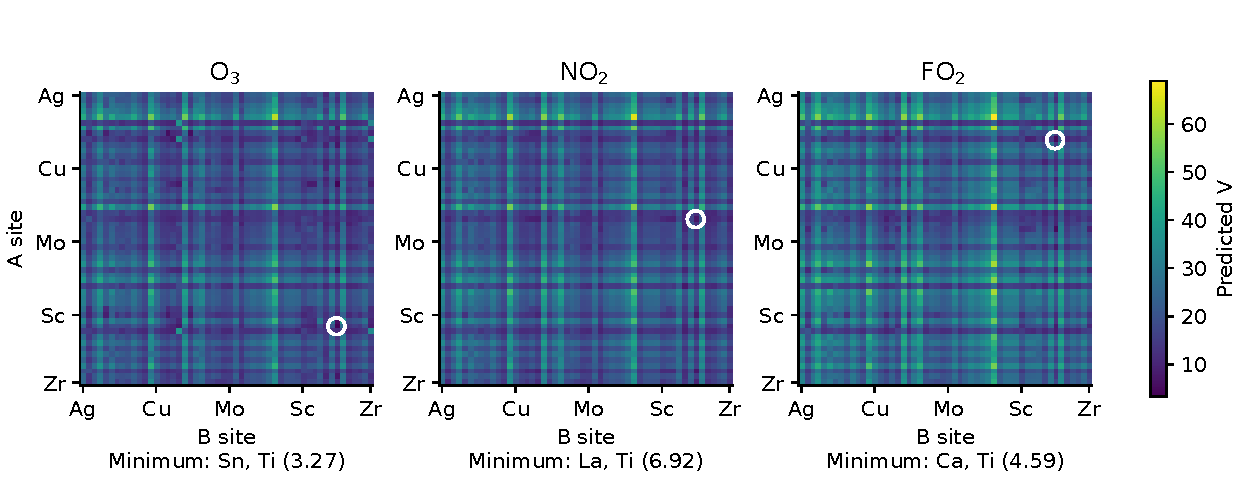
\includegraphics[width=\linewidth]{figures/family_landscapes.pdf}
\caption{Full-pool surrogate scores on the three $52\times52$ metal-pair grids. The row selects A and the column selects B. Dark colors indicate low predicted violation. The open circle marks each panel's minimum. Both axes are categorical.}\label{fig:families}
\end{figure}

The three minima share Ti on the B site and differ at A. They are $(\mathrm{Sn},\mathrm{Ti})$ at 3.268113 in O3, $(\mathrm{La},\mathrm{Ti})$ at 6.924382 in NO2, and $(\mathrm{Ca},\mathrm{Ti})$ at 4.585642 in FO2. Eight of the ten lowest scores across the full three-family pool also place Ti at B. This concentration describes the frozen surrogate. The ten records are selected extremes and cannot establish a general causal effect of Ti.

Holding La and Ti fixed, switching from NO2 to FO2 increases the score from 6.9244 to 10.1357, and switching to O3 raises it to 11.0688. Across all 2,704 pairs, however, O3 supplies the smallest score in 2,188 cells, NO2 in 378 and FO2 in 138. Each cell has a unique family minimum in the stored table. Thus choosing the family with the most pairwise wins would overlook the preferred family for the blind finalist.

The public Q3 winner also allows a physical check. Its formation energy of 0.10 eV, gap of 2.50 eV and VBM of 6.998833 eV all pass the corresponding thresholds. Its CBM of 4.518833 eV exceeds 4.50 by only 0.018833 eV, accounting for its entire reported violation. For the blind $\mathrm{LaTiO_2N}$ candidate, only composition and surrogate rank are observed. A new physical calculation would be needed to identify its limiting property.

